\documentclass[conference]{IEEEtran}
\IEEEoverridecommandlockouts

 
\newcommand{\linebreakand}{%
  \end{@IEEEauthorhalign}
  \hfill\mbox{}\par
  \mbox{}\hfill\begin{@IEEEauthorhalign}
}
\makeatother
\usepackage{cite}
\usepackage{hyperref}
\usepackage{amsmath,amssymb,amsfonts}
\usepackage{algorithmic}
\usepackage{graphicx}
\usepackage{tikz}
\usetikzlibrary{automata, positioning, arrows}
\usepackage{textcomp}
\usepackage{xcolor}
\def\BibTeX{{\rm B\kern-.05em{\sc i\kern-.025em b}\kern-.08em
    T\kern-.1667em\lower.7ex\hbox{E}\kern-.125emX}}
\begin{document}

\title{Exploring GANs and Application}

\author{\IEEEauthorblockN{Siddhant Midha}
\IEEEauthorblockA{\textit{Dept. of Electrical Engineering} \\
\textit{IIT Bombay}\\
\href{mailto:siddhantm@iitb.ac.in}{\texttt{siddhantm@iitb.ac.in}}
}
\and
\IEEEauthorblockN{Waqar Mirza}
\IEEEauthorblockA{\textit{Dept. of Electrical Engineering} \\
\textit{IIT Bombay}\\
\href{mailto:200070090@iitb.ac.in}{\texttt{200070090@iitb.ac.in}}}
\and
\IEEEauthorblockN{Dadhichi Telwadkar}
\IEEEauthorblockA{\textit{Dept. of Electrical Engineering} \\
\textit{IIT Bombay}\\
\href{mailto:20D070083@iitb.ac.in}{\texttt{20D070083@iitb.ac.in}}}
\and
\linebreakand
    \IEEEauthorblockN{Yuvraj Singh}
\IEEEauthorblockA{\textit{Dept. of Electrical Engineering} \\
\textit{IIT Bombay}\\
\href{mailto:200070093@iitb.ac.in}{\texttt{200070093@iitb.ac.in}}}


}

\maketitle

\begin{abstract}
Generative Adversarial Networks, or GANs are one among the many generative deep learning models. In this project we attempt to learn about GANs by exploring a popular application of the same, viz., image translation. The aim is, given data consisting of input image and corresponding output image we train a model such that given a another input image it generates an image which is semantically consistent with the input. Here, we take the example of colourization. Before that, we elaborate on the fundamentals of GANs, build some basic models, and finally build a translation models which performs colourization on anime faces.
\end{abstract}
\href{https://github.com/siddhant-midha/CS419M-Project}{\color{pink}\texttt{Link to GitHub Repo}\color{black}}


\section{Introduction}
We aim to understand the fundamentals of GANs through this project. We organize our work as follows -- First, we code up GANs which consist of only dense networks, hen we move on to dcGANs. Further, we take a look at conditional GANs and end the project with a GAN which performs image to image translation.
\section{What are GANs?}
A Generative Adversarial Network, or GAN is one of the many generative models that are available today. They are primarily used to estimate probability density functions \textit{implicitly} -- the main application consists of drawing samples from a given distribution. \\ 
A GAN is naturally described as a game between two players -- a \textit{generator} and a \textit{discriminator}. Given some distribution $\mathfrak{D}$, the generator tries to generate samples from the distribution, and the distributor tries to root out fake samples. That is, the generator tries to fool the discriminator and the discriminator tries to catch the generator. To ``win" this game, the generator must learn to create samples that are drawn from $\mathfrak{D}$. \\ The input to the generator is a \textit{latent variable} $z$, which is often sampled from a univariate gaussian. And the output of the generator is a desired image. Thus the generator is a function from the latent space to the image space, and the discriminator is a function from the image space to say, $[0,1]$ (that is, the decision of the discriminator).
\tikzset{
->, % makes the edges direct % makes the arrow heads bold
node distance=3cm, % specifies the minimum distance between two nodes. Change if necessary.
every state/.style={thick, fill=gray!10}, % sets the properties for each ’state’ node
initial text=$ $, % sets the text that appears on the start arrow
}
\begin{figure}[ht] % ’ht’ tells LaTeX to place the figure ’here’ or at the top of the page
\centering % centers the figure
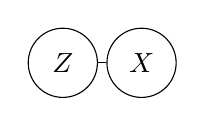
\begin{tikzpicture}
\node[state] (z) {$Z$};
\node[state, right of=z] (x) {$X$};
\draw (z) edge (x);
\end{tikzpicture}

\caption{A directed model of the generator}
\label{fig:my_label}
\end{figure}

In terms of cost functions, let $\theta_G$ and $\theta_D$ be the generator's and discriminator's parameters. And let $J_G(\theta_G,\theta_D)$ and $J_D(\theta_G,\theta_D)$ be the respective objective functions.

Now recall the goal -- 
\begin{itemize}
    \item The discriminator has to identify the real samples as real.
    \item The discriminator has to identify the generated samples as fake.
    \item The generator's aim is to fool the discriminator.
\end{itemize}
Now, let $D(x)$ be the decision of the discriminator when queried with a sample $x$ and let $G(z)$ be the output of the generator when fed with latent vector $z$. Define
     \[J_1 := \mathbb{E}_{x \sim p_{data}}log(D(x))\]
     \[J_2 := \mathbb{E}_zlog(1 - D(G(z)))\]
     \[J_3 := \mathbb{E}_zlog(D(G(z)))\]
Thus we have the generator and discriminator cost functions as
\[J_G := -J_3, J_D := -J_1 - J_2\]

Or, we can simply define $J_G$ to be $-J_D$. So if we let $V(\theta_G,\theta_D) \equiv -J_D(\theta_G,\theta_D)$, we have a min-max game as follows
 \[\min_{\theta_G}\max_{\theta_D}V(\theta_G,\theta_D)\]
There are some theoretical guarantees about the when equilibrium is attained.  In the space of arbitrary functions $G$ and $D$ a unique solutions exists such that $G$ recovers the exact distribution and $D$ is the constant function $0.5$.\newpage 


\section{Implementations and Results}

\subsection{Basic GAN}\label{AA}
First we implemented a basic GAN as a proof of concept. Here the generator and discriminator make use of dense layers (no convolutional layers) and there is no input involved to get a conditioned output. Instead the trained generator is fed only noise and outputs an image from the distribution of the training dataset. The architecture used for the generator and discriminator in various attempts will be mentioned and the results will be shown. The training methodology is as following -- In each batch of each epoch, we train the discriminator first. Then, we freeze the weights of the discriminator and train the generator.
We worked on two datasets. These are the \texttt{MNIST} dataset and the \texttt{FashionMNIST} dataset:
\subsubsection{\texttt{FashionMNIST}}
The architecture for Generator and Discriminator networks used for this dataset are as follows:

\begin{figure}[h]
\centering
\includegraphics[scale = 0.25]{dGAN_FMNIST_disc_model.png}
  \caption{Simple GAN FashionMNIST Discriminator network}
\end{figure}

\begin{figure}[h]
\centering
\includegraphics[scale = 0.25]{dGAN_FMNIST_gen_model.png}
  \caption{Simple GAN FashionMNIST Generator network}
\end{figure}

We did not make use of Batch-normalisation after different layers in this case. The GAN was trained for 20 epochs. Some images generated by the trained GAN are shown below. We can see that it performs decently and the generated images resemble the images from the training dataset and we can make out some clothing items, bags and shoes.

\begin{figure}[h]
\centering
\includegraphics[scale = 0.7]{on_f_mnist.png}
  \caption{Basic GAN results on FashionMNIST dataset}
\end{figure}

Thus this simple architecture performs rather well on this dataset. However we will soon see it performs very poorly in general and the success in this case is only due to peculiarities of this dataset.

\subsubsection{\texttt{MNIST}}
\begin{itemize}
    \item \textbf{Attempt 1:}\\
    We used the same simple GAN architecture we used for the \texttt{FashionMNIST} dataset. The network was trained for 20 epochs and the generated images by the trained network are shown. As is evident, the performance is very poor this time. All random inputs produce the same result, which appears to be a sort of mixture of the different elements of the dataset.
    
    \begin{figure}[h]
    \centering
    \includegraphics[scale = 0.6]{1st_attempt_on_mnist.png}
      \caption{Basic GAN results on MNIST dataset : Attempt 1}
    \end{figure}
    Thus this attempt gave an undesirable result.\\
    
    \item \textbf{Attempt 2:}\\
    This time we used Batch-normalisation after each layer of Generator and Discriminator except the last layers. The GAN networks used are shown.\\
    
    \begin{figure}[h]
    \centering
    \includegraphics[scale = 0.3]{dGAN_MNIST_disc_model.png}
      \caption{Simple GAN MNIST Discriminator network}
    \end{figure}
    
    \begin{figure}[h]
    \centering
    \includegraphics[scale = 0.3]{dGAN_MNIST_gen_model.png}
      \caption{Simple GAN MNIST Generator network}
    \end{figure}
    
    The results after training for 20 epochs and 50 epochs are shown. We can see a significant improvement after adding batch normalisation to the simple model.
     \begin{figure}[h]
    \centering
    \includegraphics[scale = 0.6]{2nd_attempt_mnist_20epoc.png}
      \caption{Basic GAN results on MNIST dataset : Attempt 2, 20 epochs}
    \end{figure}
     \begin{figure}[h]
    \centering
    \includegraphics[scale = 0.6]{2nd_attempt_mnist_50epoc.png}
      \caption{Basic GAN results on MNIST dataset : Attempt 2, 50 epochs}
    \end{figure}
\end{itemize}

So we have been able to test out this basic GAN model and it performs decently well on the \texttt{FashionMNIST} dataset but not so well on the \texttt{MNIST} dataset.\\
Now let us move to a slightly more complex GAN architecture.

\subsection{Convolutional GAN}
In the convolutional GAN we make use of convolutional layers in the Generator and Discriminator networks along with the dense layers. The overall training methodology remains the same. This time too we do not have an input conditioned output. The results on \texttt{MNIST} and \texttt{FashionMNIST} are discussed.\\

\begin{figure}[h]
\centering
\includegraphics[scale = 0.5]{convGAN_MNIST_20epoc.png}
  \caption{convGAN results on MNIST dataset}
\end{figure}

\subsubsection{\texttt{MNIST}}
The Generator and Discriminator training models used are shown. We have made full use of Batch-normalisation as it produced results on this dataset.\\

\begin{figure}[h]
\centering
\includegraphics[scale = 0.25]{convGAN_MNIST_disc_model.png}
  \caption{convGAN MNIST Discriminator network}
\end{figure}

\begin{figure}[h]
\centering
\includegraphics[scale = 0.25]{convGAN_MNIST_gen_model.png}
  \caption{convGAN MNIST Generator network}
\end{figure}

The convGAN was trained for 20 epochs on the dataset and the results produced are shown. We can see that the performance of convGAN on MNIST dataset is very good, in contrast with the case of the basic GAN. Use of batchnormalisation is seen to work well with this dataset.\\

\subsubsection{\texttt{FashionMNIST}}

\begin{itemize}
    \item \textbf{Attempt 1:}\\
    We used the same convGAN architecture we used for the \texttt{MNIST} dataset. The generated images are shown for a training of both 20 epochs and 50 epochs. As is evident, the performance is very poor this time, and the outputs don't resemble the dataset elements.
    
    \begin{figure}[h]
    \centering
    \includegraphics[scale = 0.5]{convGAN_FashionMNIST_20epoc (bad).png}
      \caption{convGAN results on FashionMNIST dataset : Attempt 1, 20 epochs}
    \end{figure}
    
    \begin{figure}[h]
    \centering
    \includegraphics[scale = 0.5]{convGAN_FashionMNIST_50epoc (bad).png}
      \caption{convGAN results on FashionMNIST dataset : Attempt 1, 50 epochs}
    \end{figure}
    
    Thus this attempt gave an undesirable result.\\
    \newpage
    \item \textbf{Attempt 2:}\\
    This time we reduce the use Batch-normalisation between layers, which surprisingly seems to improve results on this dataset. The GAN networks used are shown.\\
    
    \begin{figure}[h]
    \centering
    \includegraphics[scale = 0.3]{convGAN_FMNIST_disc_model.png}
      \caption{convGAN FashionMNIST Discriminator network : Attempt 2}
    \end{figure}
    
    \begin{figure}[h]
    \centering
    \includegraphics[scale = 0.3]{convGAN_FMNIST_gen_model.png}
      \caption{convGAN FashionMNIST Generator network : Attempt 2}
    \end{figure}\\

   \begin{figure}[h]
    \centering
    \includegraphics[scale = 0.6]{convGAN_FashionMNIST_20epoc_LESSBNORM (less bad).png}
      \caption{Basic GAN results on MNIST dataset : Attempt 2, 20 epochs}
    \end{figure}
     \begin{figure}[h]
    \centering
    \includegraphics[scale = 0.6]{convGAN_FashionMNIST_50epoc_LESSBNORM (nice).png}
      \caption{Basic GAN results on MNIST dataset : Attempt 2, 50 epochs}
    \end{figure}
    
    The results after training for 20 epochs and 50 epochs are shown.\\
    In this case there is an improvement over attempt 1. Moreover, the outputs seem to be biased towards shoes. We can see that the performance of the convGAN is much worse than our basic GAN on this dataset, which is indeed a peculiar feature of this dataset, alongwith the observation that reducing Batch-normalisation works better with this dataset.
\end{itemize}
Now we move to a conditional GAN.

\subsection{condGAN}
We created condGAN models for both the \texttt{MNIST} and \texttt{FashionMNIST} datasets. In a conditional GAN the Generator takes an external input along with the noise. The input specifies the class label of the output the generator needs to generate, and the trained generator needs to sample an output from the distribution of that class. The discriminator takes the class vector and the generator output as inputs. We have 10 classes in both datasets, so we use one hot encoding and the class vector has size 10. Since the generator has output with one dimension as 28, we concatenate a repeated $28\times 10$ matrix with rows as class vector with the generator output and feed it to discriminator. We can see that this cannot be a sequential model as the input (class) vector is fed to both generator and discriminator. For the generator the class vector and latent vector (noise vector) are concatenated and fed as input. As we could not form a composite GAN model using generator and discriminator models in the condGAN (as we needed to take the class label as an input too), we trained discriminator and generator separately and used the \texttt{tf.GradientTape} method for training the generator.\\
The models for generator and discriminator (used on both datasets) are shown.

\begin{figure}[h]
\centering
\includegraphics[scale = 0.25]{condGAN_disc_model.png}
  \caption{condGAN Discriminator model}
\end{figure}

\begin{figure}[h]
\centering
\includegraphics[scale = 0.25]{condGAN_gen_model.png}
  \caption{condGAN FashionMNIST Generator model}
\end{figure}\\

\textbf{Results:}\\
After training for 20 epochs, the generated images for different classes are shown for the two datasets. Here each row of the results corresponds to one class query with different latent vectors. Note that (i) \texttt{MNIST} dataset did NOT require additional Batch-normalisation to produce good results, (ii) \texttt{FashionMNIST} trained much faster than \texttt{MNIST}.
\begin{figure}[h]
\centering
\includegraphics[scale = 0.5]{condGAN_MNIST_20epoc.png}
  \caption{Conditional GAN results on MNIST dataset, 20 epochs}
\end{figure}
 \begin{figure}[h]
\centering
\includegraphics[scale = 0.5]{condGAN_Fashion_20epoc.png}
  \caption{Conditional GAN results on FashionMNIST dataset, 20 epochs}
\end{figure}\\
We can see that the GAN performs very well here.
\newpage 
\subsection{Image Translation using condGAN : Anime Colourization}
\noindent 
After exploring basic GAN models, we now aim to work on an application of the same. Taking inspiration from $condGAN$ and some affinity towards anime, we implement a GAN model to colourize anime characters. \\ 
We use a conditional GAN to learn to colour an anime character given its uncoloured version, by training on data from \href{https://www.kaggle.com/datasets/ktaebum/anime-sketch-colorization-pair}{\texttt{anime-sketch-colorization-pair}} dataset on Kaggle.\\ In this case, the Generator takes the mask which is $256\times256\times3$ image of the sketch, passes it via combination of upsample and downsample blocks to generate coloured image of given sketch. The Discriminator identifies if the image is real or fake(generated), doesn't use noise for initialisation.\\
The results on a sample input image as the model is trained for different number of epochs are shown. 
\begin{figure}[h]
\centering
\includegraphics[scale = 0.25]{0ep.png}
  \caption{Result : 0 epochs}
\end{figure}

\begin{figure}[h]
\centering
\includegraphics[scale = 0.25]{10ep.png}
  \caption{Result : 10 epochs}
\end{figure}

\begin{figure}[h]
\centering
\includegraphics[scale = 0.25]{20ep.png}
  \caption{Result : 20 epochs}
\end{figure}

\begin{figure}[h]
\centering
\includegraphics[scale = 0.25]{30ep.png}
  \caption{Result : 30 epochs}
\end{figure}

\begin{figure}[h]
\centering
\includegraphics[scale = 0.25]{40ep.png}
  \caption{Result : 40 epochs}
\end{figure}
\newpage
\begin{figure}[h]
\centering
\includegraphics[scale = 0.25]{50ep.png}
  \caption{Result : 50 epochs}
\end{figure}
\begin{figure}[h]
\centering
\includegraphics[scale = 0.25]{60ep.png}
  \caption{Result : 60 epochs}
\end{figure}

\begin{thebibliography}{00}
\bibitem{gan1}Ian J. Goodfellow, Jean Pouget-Abadie
, Mehdi Mirza, Bing Xu, David Warde-Farley,
Sherjil Ozair
, Aaron Courville, Yoshua Bengio, ``Generative Adversarial Nets", \href{https://arxiv.org/pdf/1406.2661.pdf}{\texttt{https://arxiv.org/pdf/1406.2661.pdf}}
\bibitem{condgan}Mehdi Mirza, Simon Osindero, ``Conditional Generative Adversarial Nets
", \href{https://arxiv.org/pdf/1411.1784.pdf}{\texttt{https://arxiv.org/pdf/1411.1784.pdf}}
\bibitem{gantut}Ian Goodfellow ``NIPS 2016 Tutorial:
Generative Adversarial Networks" \href{https://arxiv.org/pdf/1701.00160.pdf}{\texttt{https://arxiv.org/pdf/1701.00160.pdf}}
\end{thebibliography}
\end{document}
